\documentclass{beamer} % Beamer document class for presentations
\usetheme[secheader]{Boadilla} % Theme for the presentation
% \setbeamertemplate{navigation symbols}{} % Remove navigation symbols
\usepackage{tcolorbox} % For colored boxes and text
\usepackage{tikz} % For drawing graphics and diagrams
\usepackage{mwe} % For including example pictures (used in this document)
\usepackage{siunitx} % For typesetting SI units
\usepackage{hyperref} % For hyperlinks
%\usepackage[table]{xcolor} % For coloring tables
% Additional packages for TikZ and related features
\usepackage{tikz}
\usepackage{tcolorbox}
\definecolor{BrockRed}{RGB}{204,0,0} % Brock Red
% \usecolortheme[named=BrockRed]{structure}
\usecolortheme{beaver}
\usepackage{colortbl} % For colored cells in tables
\usepackage{xcolor} % For defining custom colors
\usepackage{graphicx} % For \cellcolor command
\usetikzlibrary{positioning, arrows.meta} % Additional TikZ libraries for positioning and arrow styles
\usepackage{color} % For custom color definitions
\usepackage{epsfig} % For EPS figures
\usepackage{ifpdf} % For conditional checks based on output format
\usepackage[latin1]{inputenc} % Input encoding
\usepackage{multimedia} % For including multimedia elements in presentations
\usepackage{svg}

% Define custom colors
\definecolor{Mahogany}{cmyk}{0,0.85,0.87,0.35}
\definecolor{Mahogany}{RGB}{43,117,22}

% Additional packages for mathematical typesetting and symbols
\usepackage{latexsym}
\usepackage{amsmath,amsthm,amssymb} % For mathematical environments and symbols
\usepackage{amsmath}
\usepackage{mathrsfs} % For additional math fonts

\usepackage{listings} % For typesetting code
\usepackage{xcolor}   % For customizing colors

% Define colors for code highlighting
\definecolor{mygreen}{RGB}{0,128,0}
\definecolor{mygray}{RGB}{128,128,128}
\definecolor{mymauve}{RGB}{128,0,128}

% Define the style for Python code
\lstset{
  language=Python,
  basicstyle=\normalsize\ttfamily,
  keywordstyle=\color{blue},
  commentstyle=\color{mygreen},
  numberstyle=\tiny\color{mygray},
  stringstyle=\color{mymauve},
  breaklines=true,
  breakatwhitespace=true,
  %numbers=left,
  frame=single,
  showstringspaces=false,
  captionpos=b,
}


\definecolor{darkred}{rgb}{139, 0, 0}
\ifpdf
  \DeclareGraphicsExtensions{.png,.pdf}
\else
  \DeclareGraphicsExtensions{.eps}
\fi



%%%%%%%%%%%%%%%%%%%%%% title page %%%%%%%%%%%%%%%%%%%%%%%%%%%%%

% Set the short title for the presentation (appears in the header)
\title[\textcolor{red}{Presentation Title}]{\textbf{Presentation Title}}

% Set the author information with a colored name (appears in the footer)
\author[\textcolor{white}{Presenter Name}]{{\Large\textcolor{red}{Presenter Name}}}
\vspace{0.5cm}
%\large{Supervised by
%\textbf{Your Supervisor Name}}}
% Define a command to set the frame author (date in this case)
\newcommand{\frameauthor}[1]{\date{#1}}

% Set the institute information with a colored short university name (appears in the footer)
\institute[\textcolor{white}{Brock University}]{
Department Name or Affiliations}

% Set the date of the presentation (today's date in this case)
\date{}
\logo{
\includegraphics[height=1cm]{Figures/BrockU-2022-RGB-Top-1050x636.jpg}}

%%%%%%%%%%%%%%%%%%%%%%%%% end title page %%%%%%%%%%%%%%%%%%%%%%%%


\AtBeginSubsection[] {
  \begin{frame}<beamer>
%    \frametitle{Abstract}
    \tableofcontents[currentsection,currentsection]
  \end{frame}
}
%%%%%%%%%%%%%%%%%%%%%%%%%%%%%%%%%%%%%%%%%%%%%%%%
%%%%%%%%%%%%%%%%%%%%%%%%%%%%%%%%%%%%%%%%%%%%%%%%
%%%%%%%%%%%%%%%%%%%%%%%%%%%%%%%%%%%%%%%%%%%%%%%%
% zaciname
%%%%%%%%%%%%%%%%%%%%%%%%%%%%%%%%%%%%%%%%%%%%%%%%
%%%%%%%%%%%%%%%%%%%%%%%%%%%%%%%%%%%%%%%%%%%%%%%%
%%%%%%%%%%%%%%%%%%%%%%%%%%%%%%%%%%%%%%%%%%%%%%%%

\begin{document}
%{\footnotesize{
%%%%%%%%%%%%%%%%%%%%%%%%%%%%%%%%%%%%%%%%%%%%%%%%
%%%%%%%%%%%%%%%%%%%%%%%%%%%%%%%%%%%%%%%%%%%%%%%%
%%%%%%%%%%%%%%%%%%%%%%%%%%%%%%%%%%%%%%%%%%%%%%%%%%
%\begin{frame}
%\includegraphics[width=\linewidth]{}
%\end{frame}
%%%%%%%%%%%%%%%%%%%%%%%%%%%%%%%%%%%%%%%%%%%%%%%%%%
%%%%%%%%%%%%%%%%%%%%%%%%%%%%%%%%%%%%%%%%%%%%%%%%%%
%%%%%%%%%%%%%%%%%%%%%%%%%%%%%%%%%%%%%%%%%%%%%%%%
\begin{frame}
  \titlepage
\end{frame}
%%%%%%%%%%%%%%%%%%%%%%%%%%%%%%%%%%%%%%%%%%%
%%%%%%%%%%%%%%%%%%%%%%%%%%%%%%%%%%%%%%%%%%%
%%%%%%%%%%%%%%%%%%%%%%%%%%%%%%%%%%%%%%%%%%
\begin{frame}\frametitle{Outline}
  \tableofcontents[hideallsubsections]
\end{frame}
%%%%%%%%%%%%%%%%%%%%%%%%%%%%%%%%%%%%%%%%%%%
%%%%%%%%%%%%%%%%%%%%%%%%%%%%%%%%%%%%%%%%%%%
%%%%%%%%%%%%%%%%%%%%%%%%%%%%%%%%%%%%%%%%%%
\section{Introduction}
    \begin{frame}[plain]
        \vfill
      \centering
      \begin{beamercolorbox}[sep=8pt,center,shadow=true,rounded=true]{title}
        \usebeamerfont{title}\insertsectionhead\par%
        \color{blue}\noindent\rule{10cm}{1pt}
      \end{beamercolorbox}
      \vfill
  \end{frame}
\begin{frame}{Title}
    \begin{itemize}
        \item Bullet Point 1
        \item Bullet Point 2
        \begin{enumerate}
            \item Sub Bullet Point 1
            \item Sub Bullet Point 2
            \item Sub Bullet Point 3
        \end{enumerate}
        \item \lipsum[1][1] \cite{nsga2}.
        \item \lipsum[1][2] \cite{nsga2}.
        \item \lipsum[1][3] \cite{nsga2}.
    \end{itemize} 
\end{frame}

\section{Section 2}
    \begin{frame}[plain]
        \vfill
      \centering
      \begin{beamercolorbox}[sep=8pt,center,shadow=true,rounded=true]{title}
        \usebeamerfont{title}\insertsectionhead\par%
        \color{orange}\noindent\rule{10cm}{1pt}
      \end{beamercolorbox}
      \vfill
  \end{frame}

\begin{frame}{Title}
\begin{itemize}
    \item \lipsum[1][1].
    \begin{align}
        \text{Minimize:} \ {f_{1}(x), f_{2}(x), ..., f_{m}(x)} \nonumber \\
        \text{Subject to:} \ g_j(x) \leq 0,\ j=0,1,...,n
    \end{align}
\end{itemize}
\end{frame}

\begin{frame}{Title}
\begin{columns}[T]
    \begin{column}{.45\textwidth}
        \begin{figure}
        \centering
        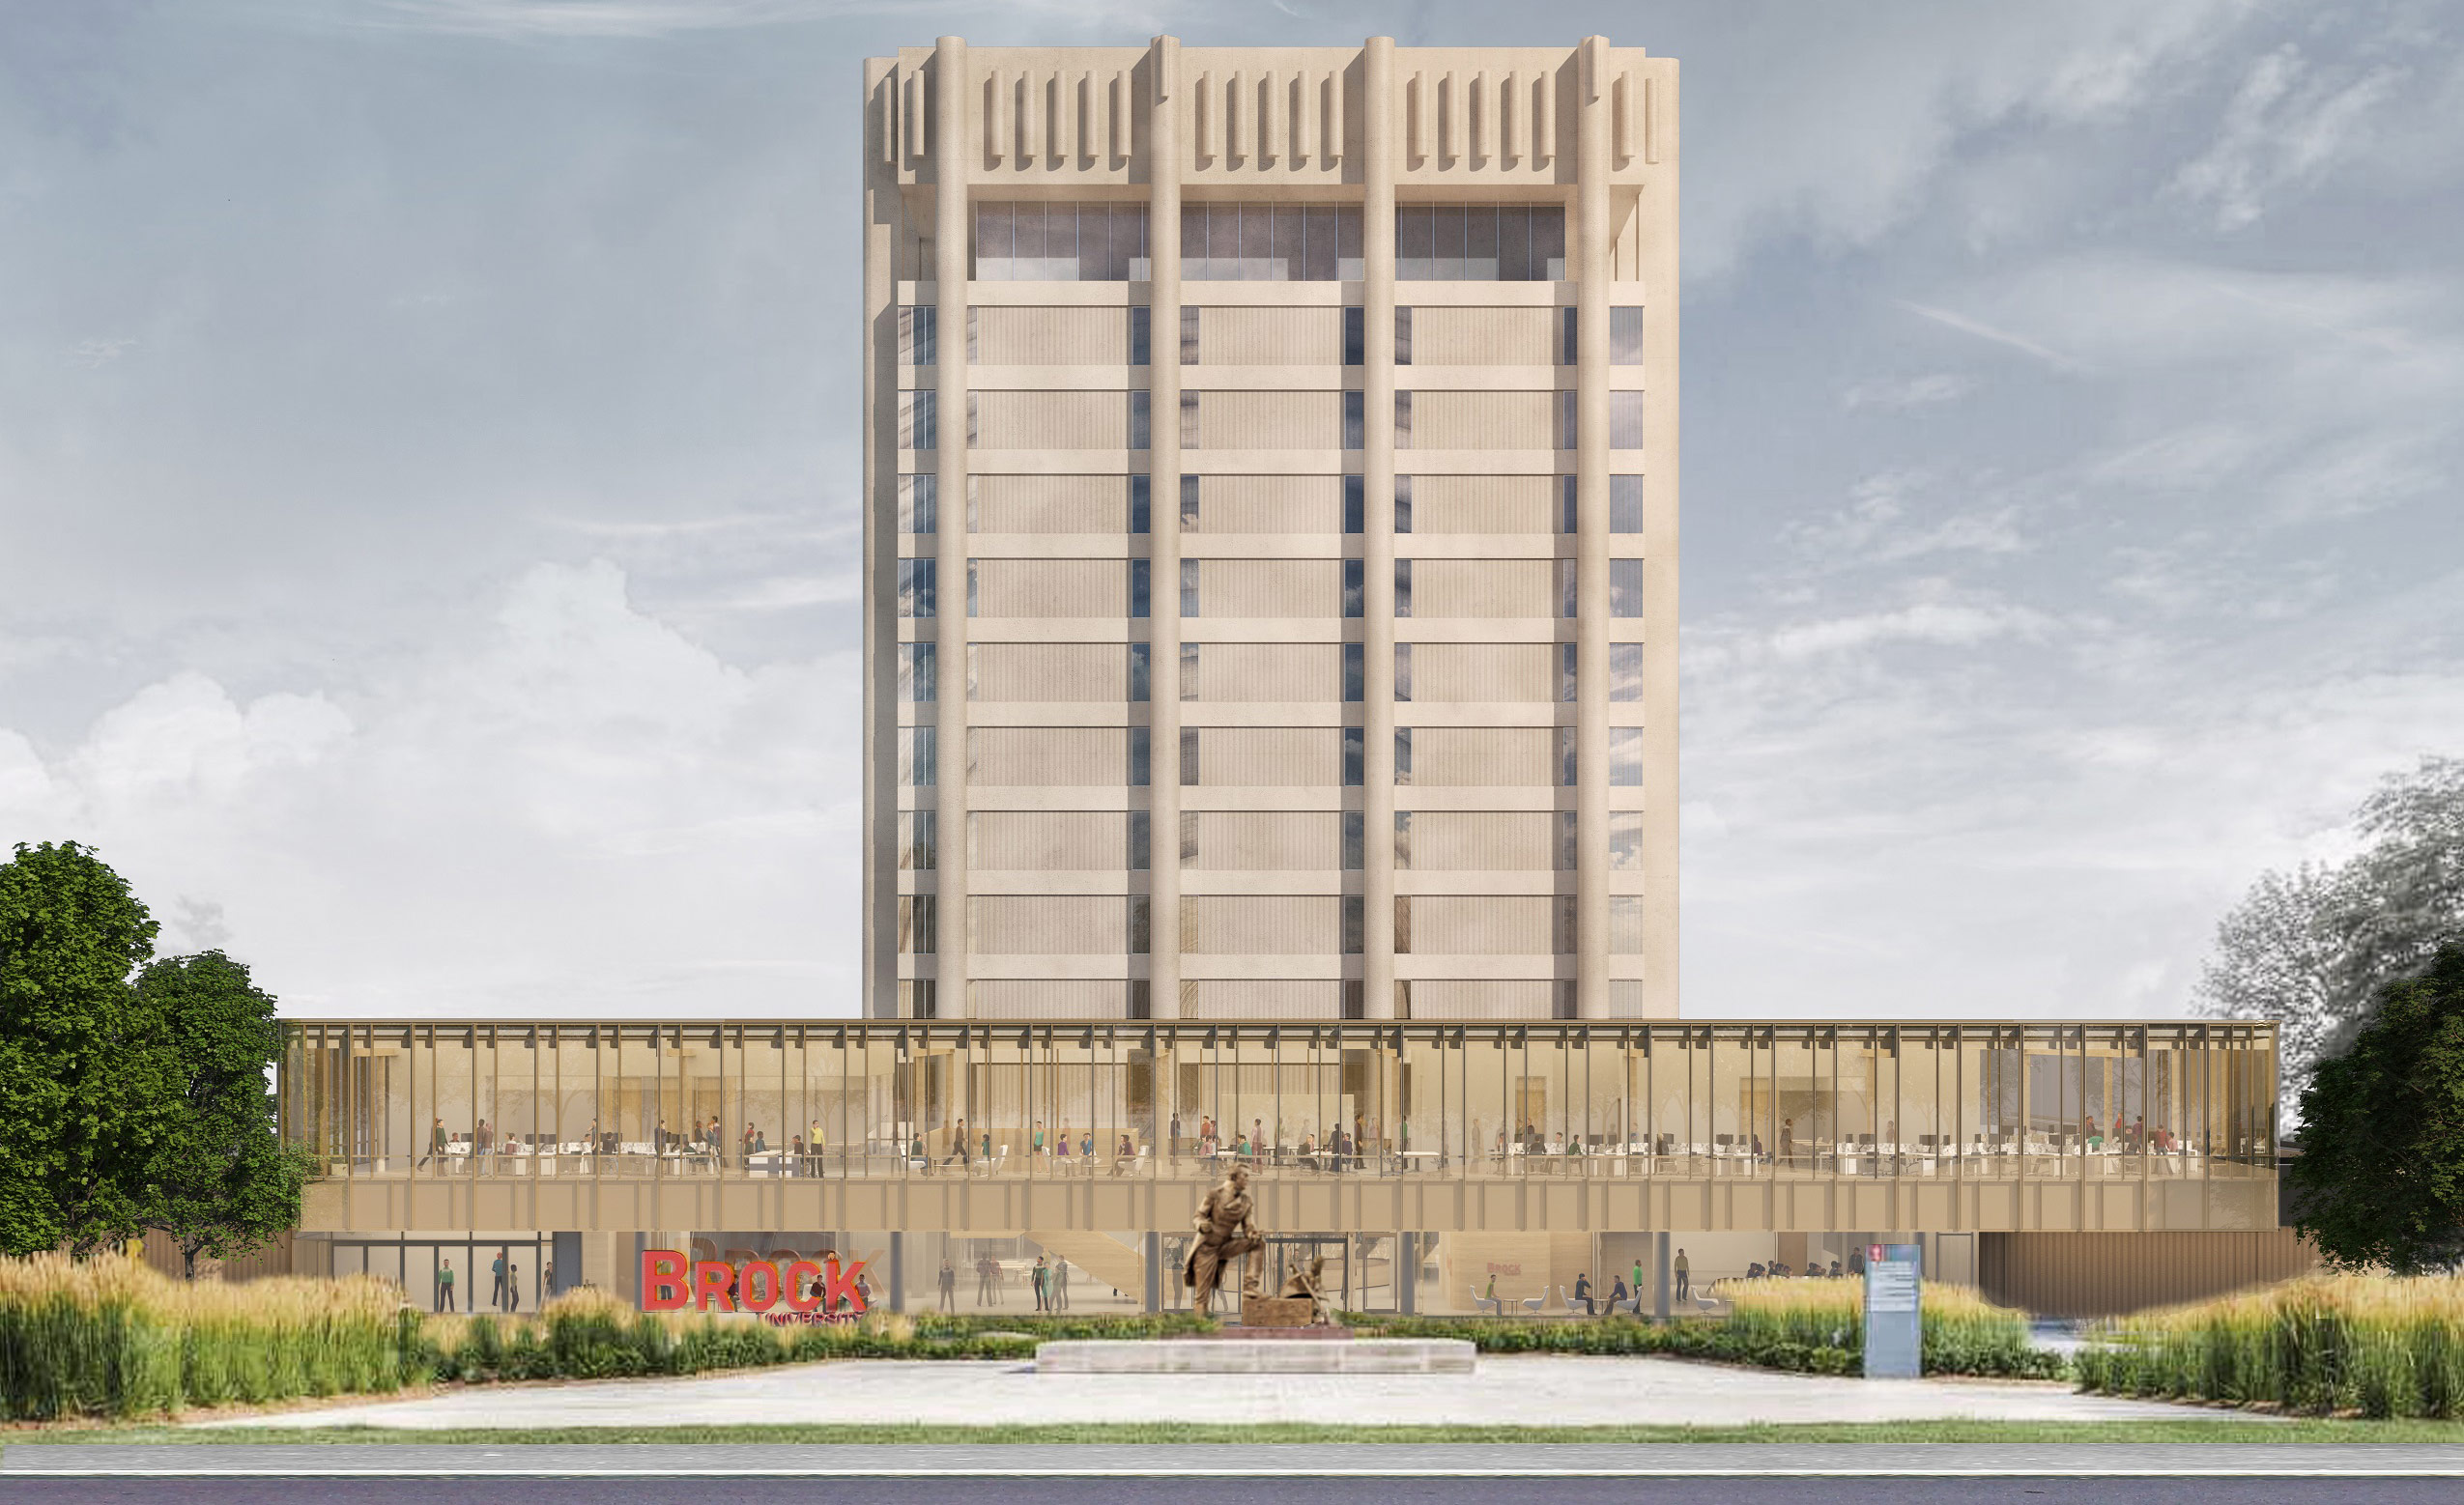
\includegraphics[scale=0.05]{Figures/Brock-LINC-Project-South-Elevation.jpg}
        \caption{Caption.}
        \label{fig:label1}
        \end{figure}
    \end{column}
    \begin{column}{.48\textwidth}
        \begin{figure}
            \centering
            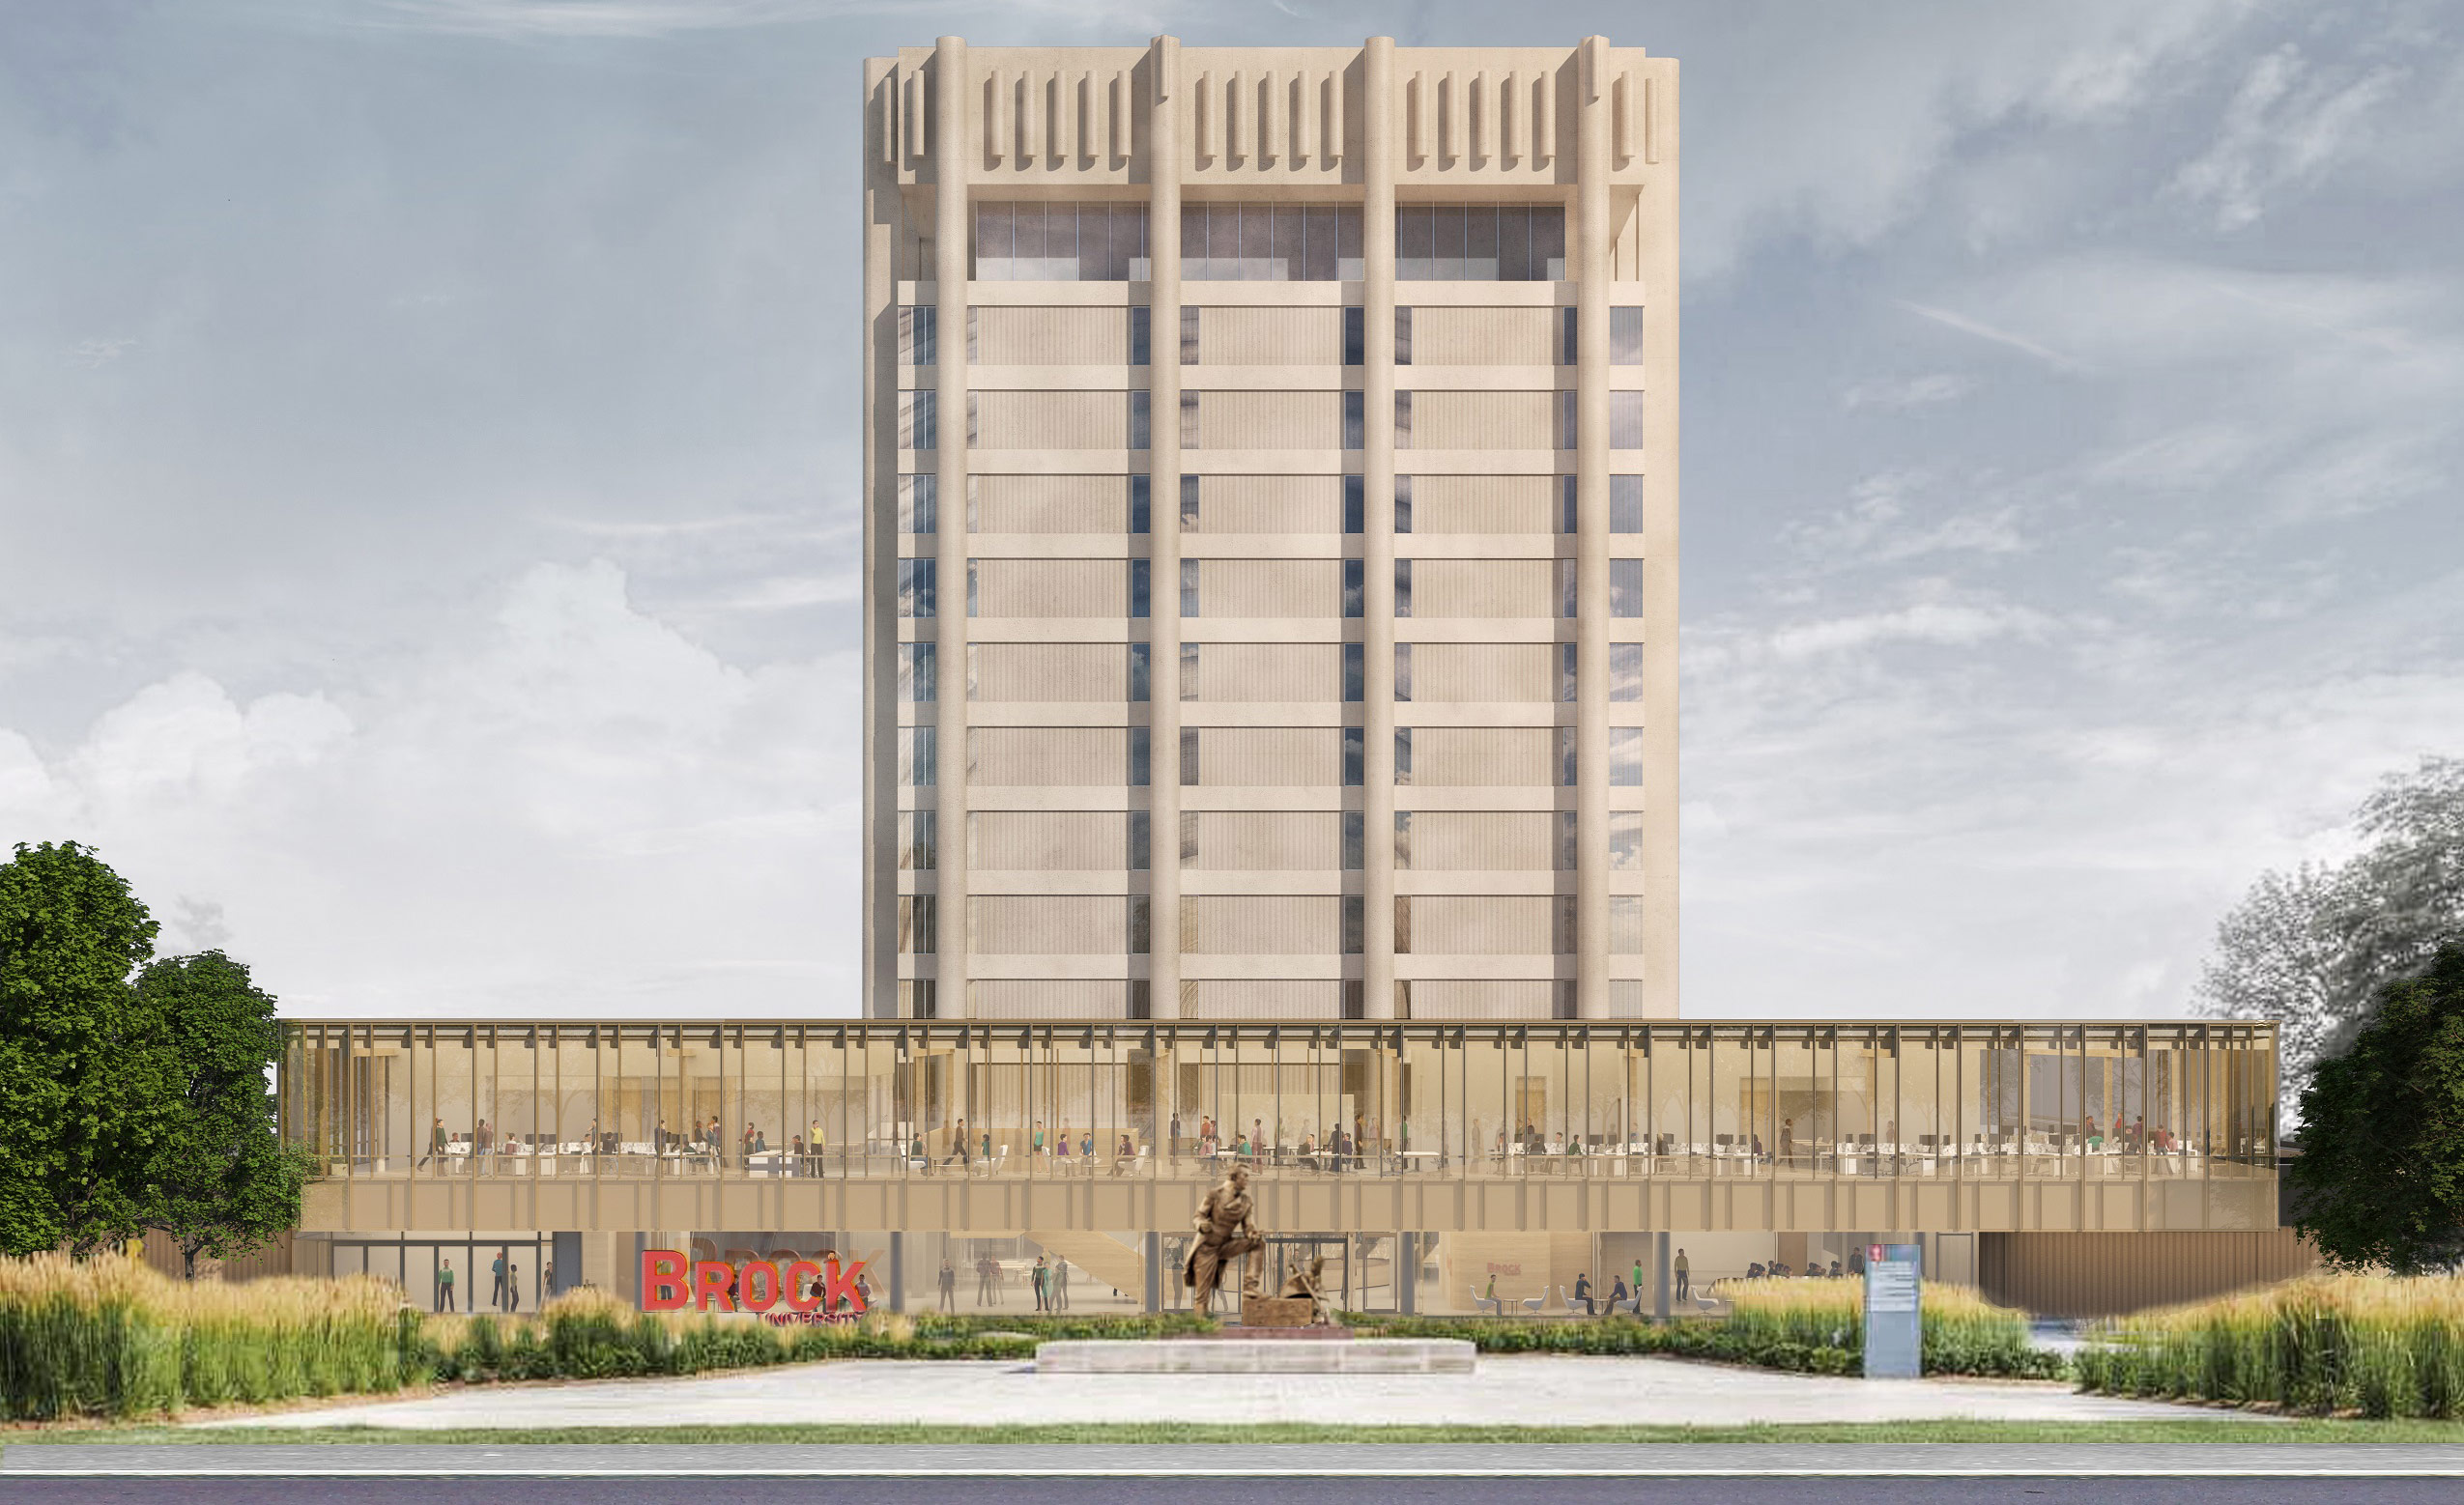
\includegraphics[scale=0.05]{Figures/Brock-LINC-Project-South-Elevation.jpg}
            \caption{Caption.}
            \label{fig:label2}
        \end{figure}
    \end{column}
\end{columns}

\end{frame}

\begin{frame}{Title}
\begin{columns}[T]
    \begin{column}{.45\textwidth}
        \begin{figure}
        \centering
        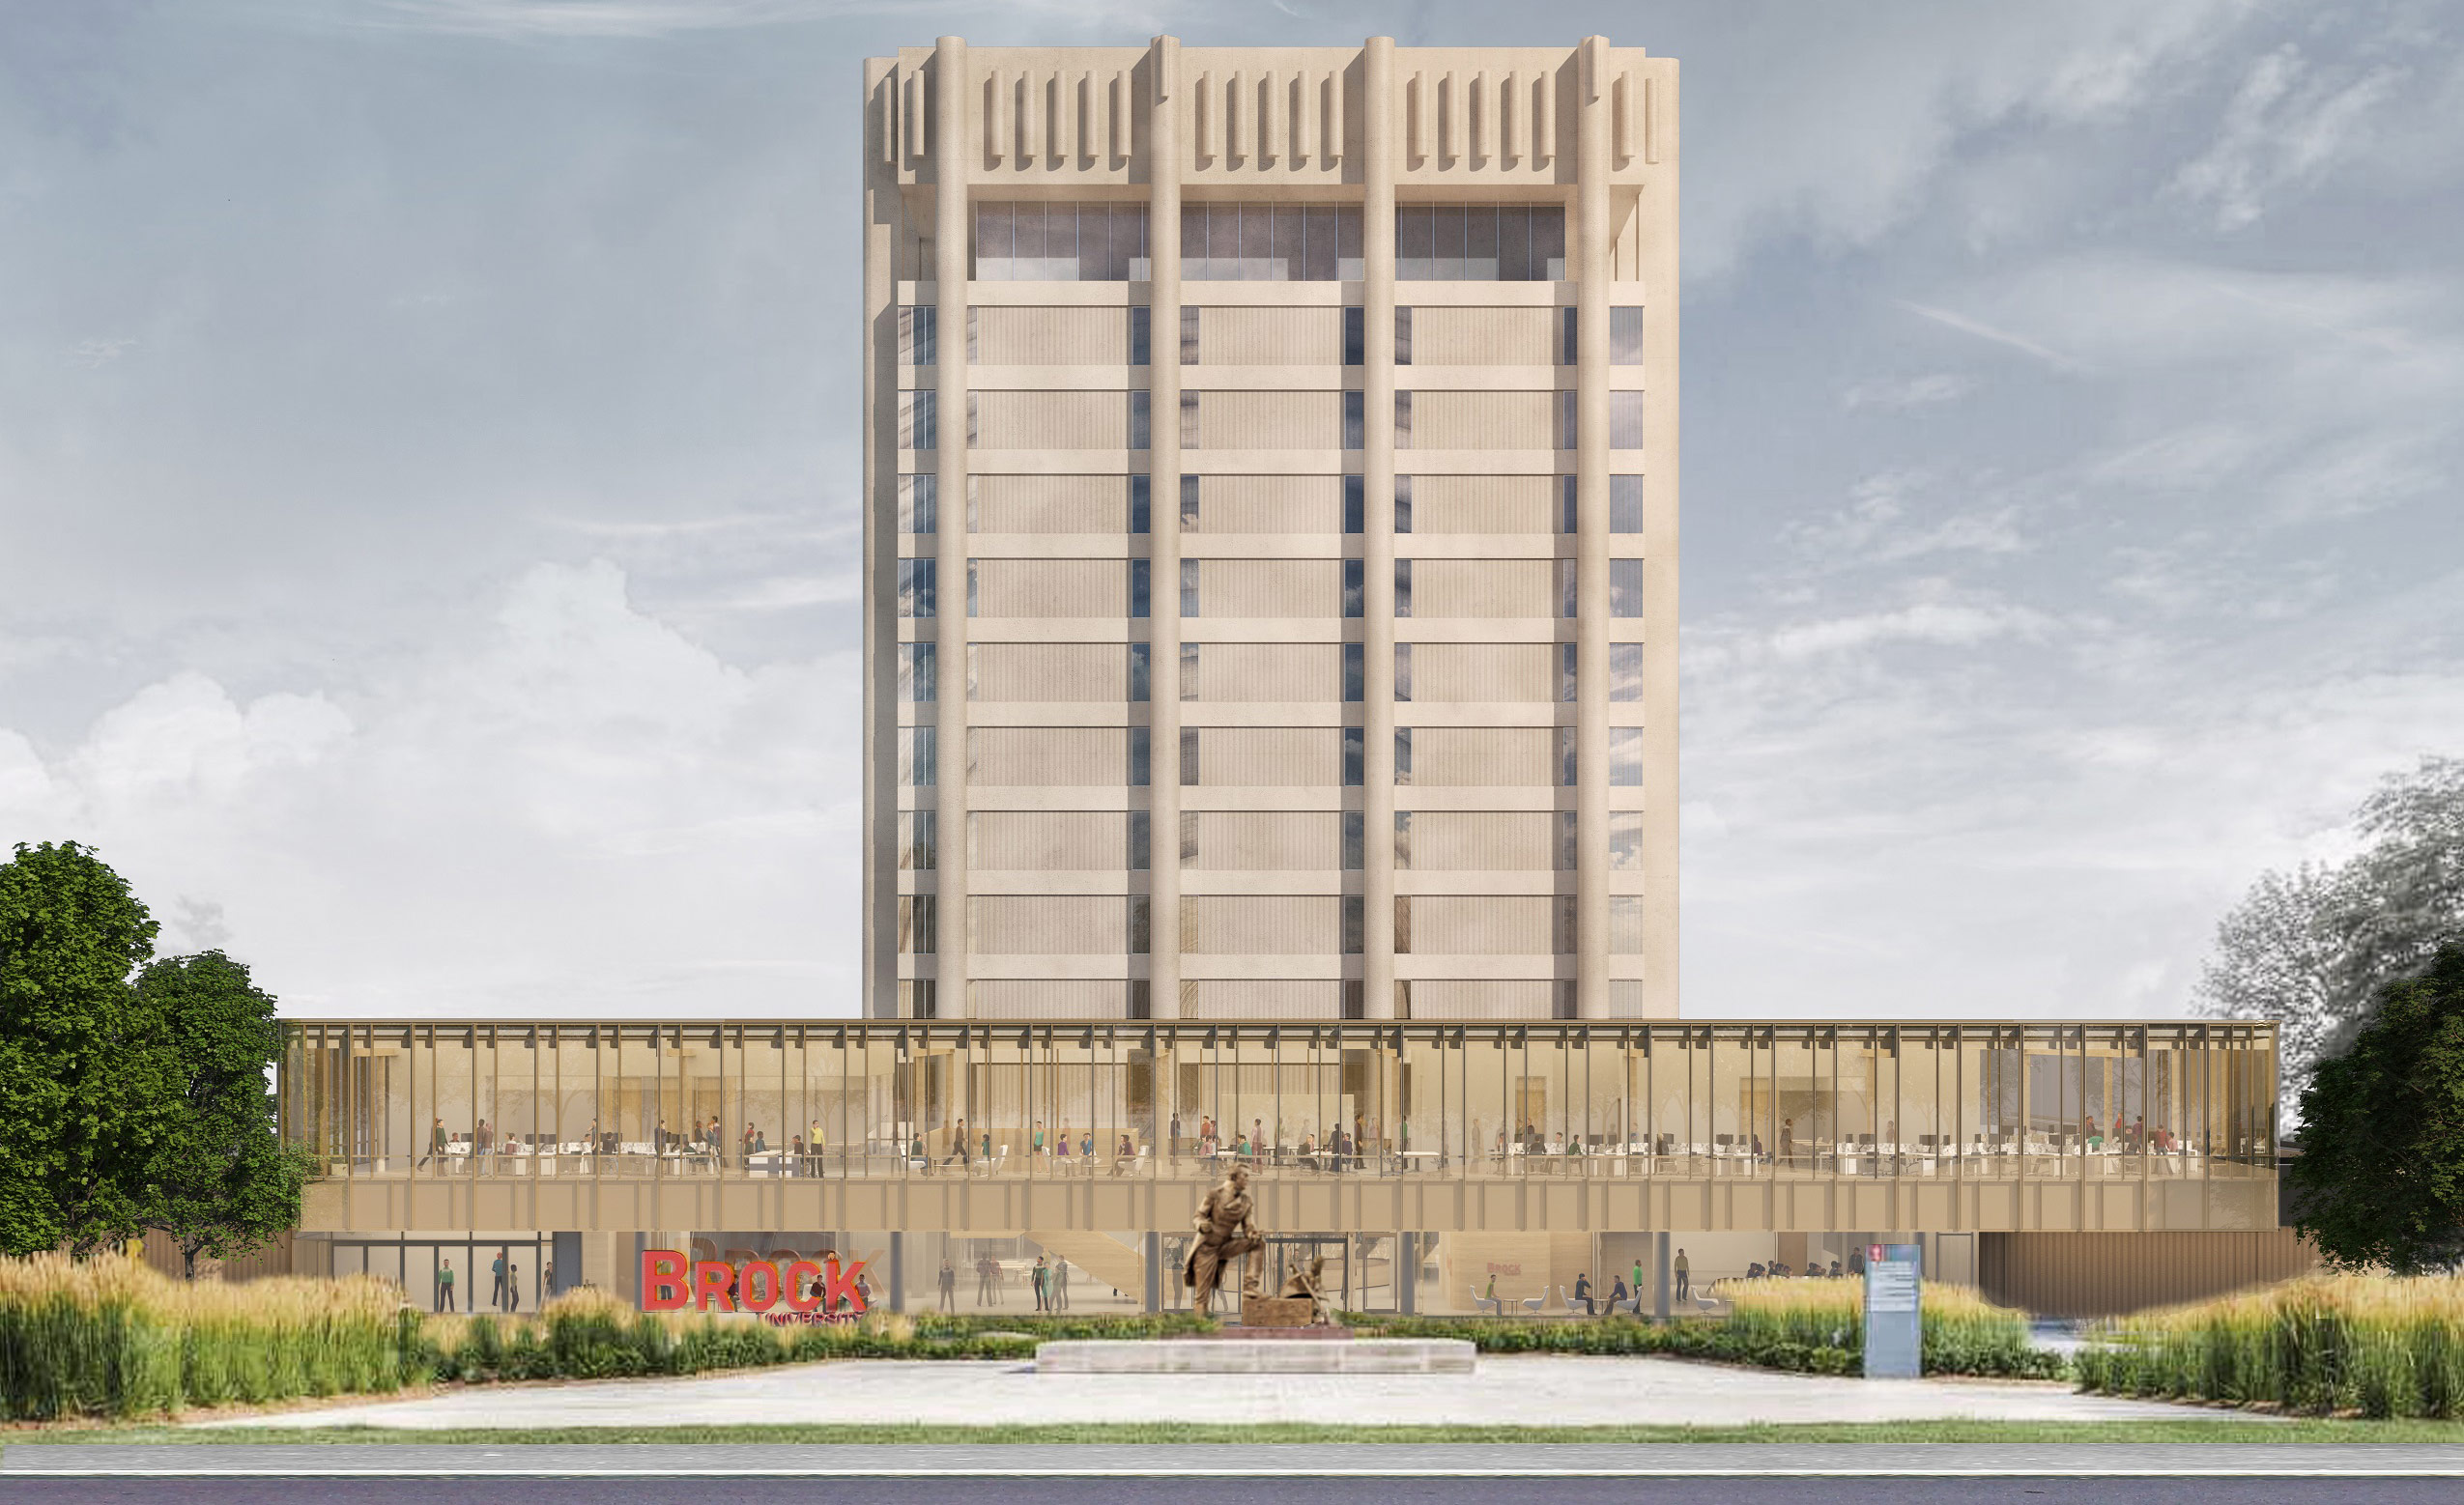
\includegraphics[scale=0.05]{Figures/Brock-LINC-Project-South-Elevation.jpg}
        \caption{Caption.}
        \label{fig:label1}
        \end{figure}
    \end{column}
    \begin{column}{.48\textwidth}
        \begin{figure}
            \centering
            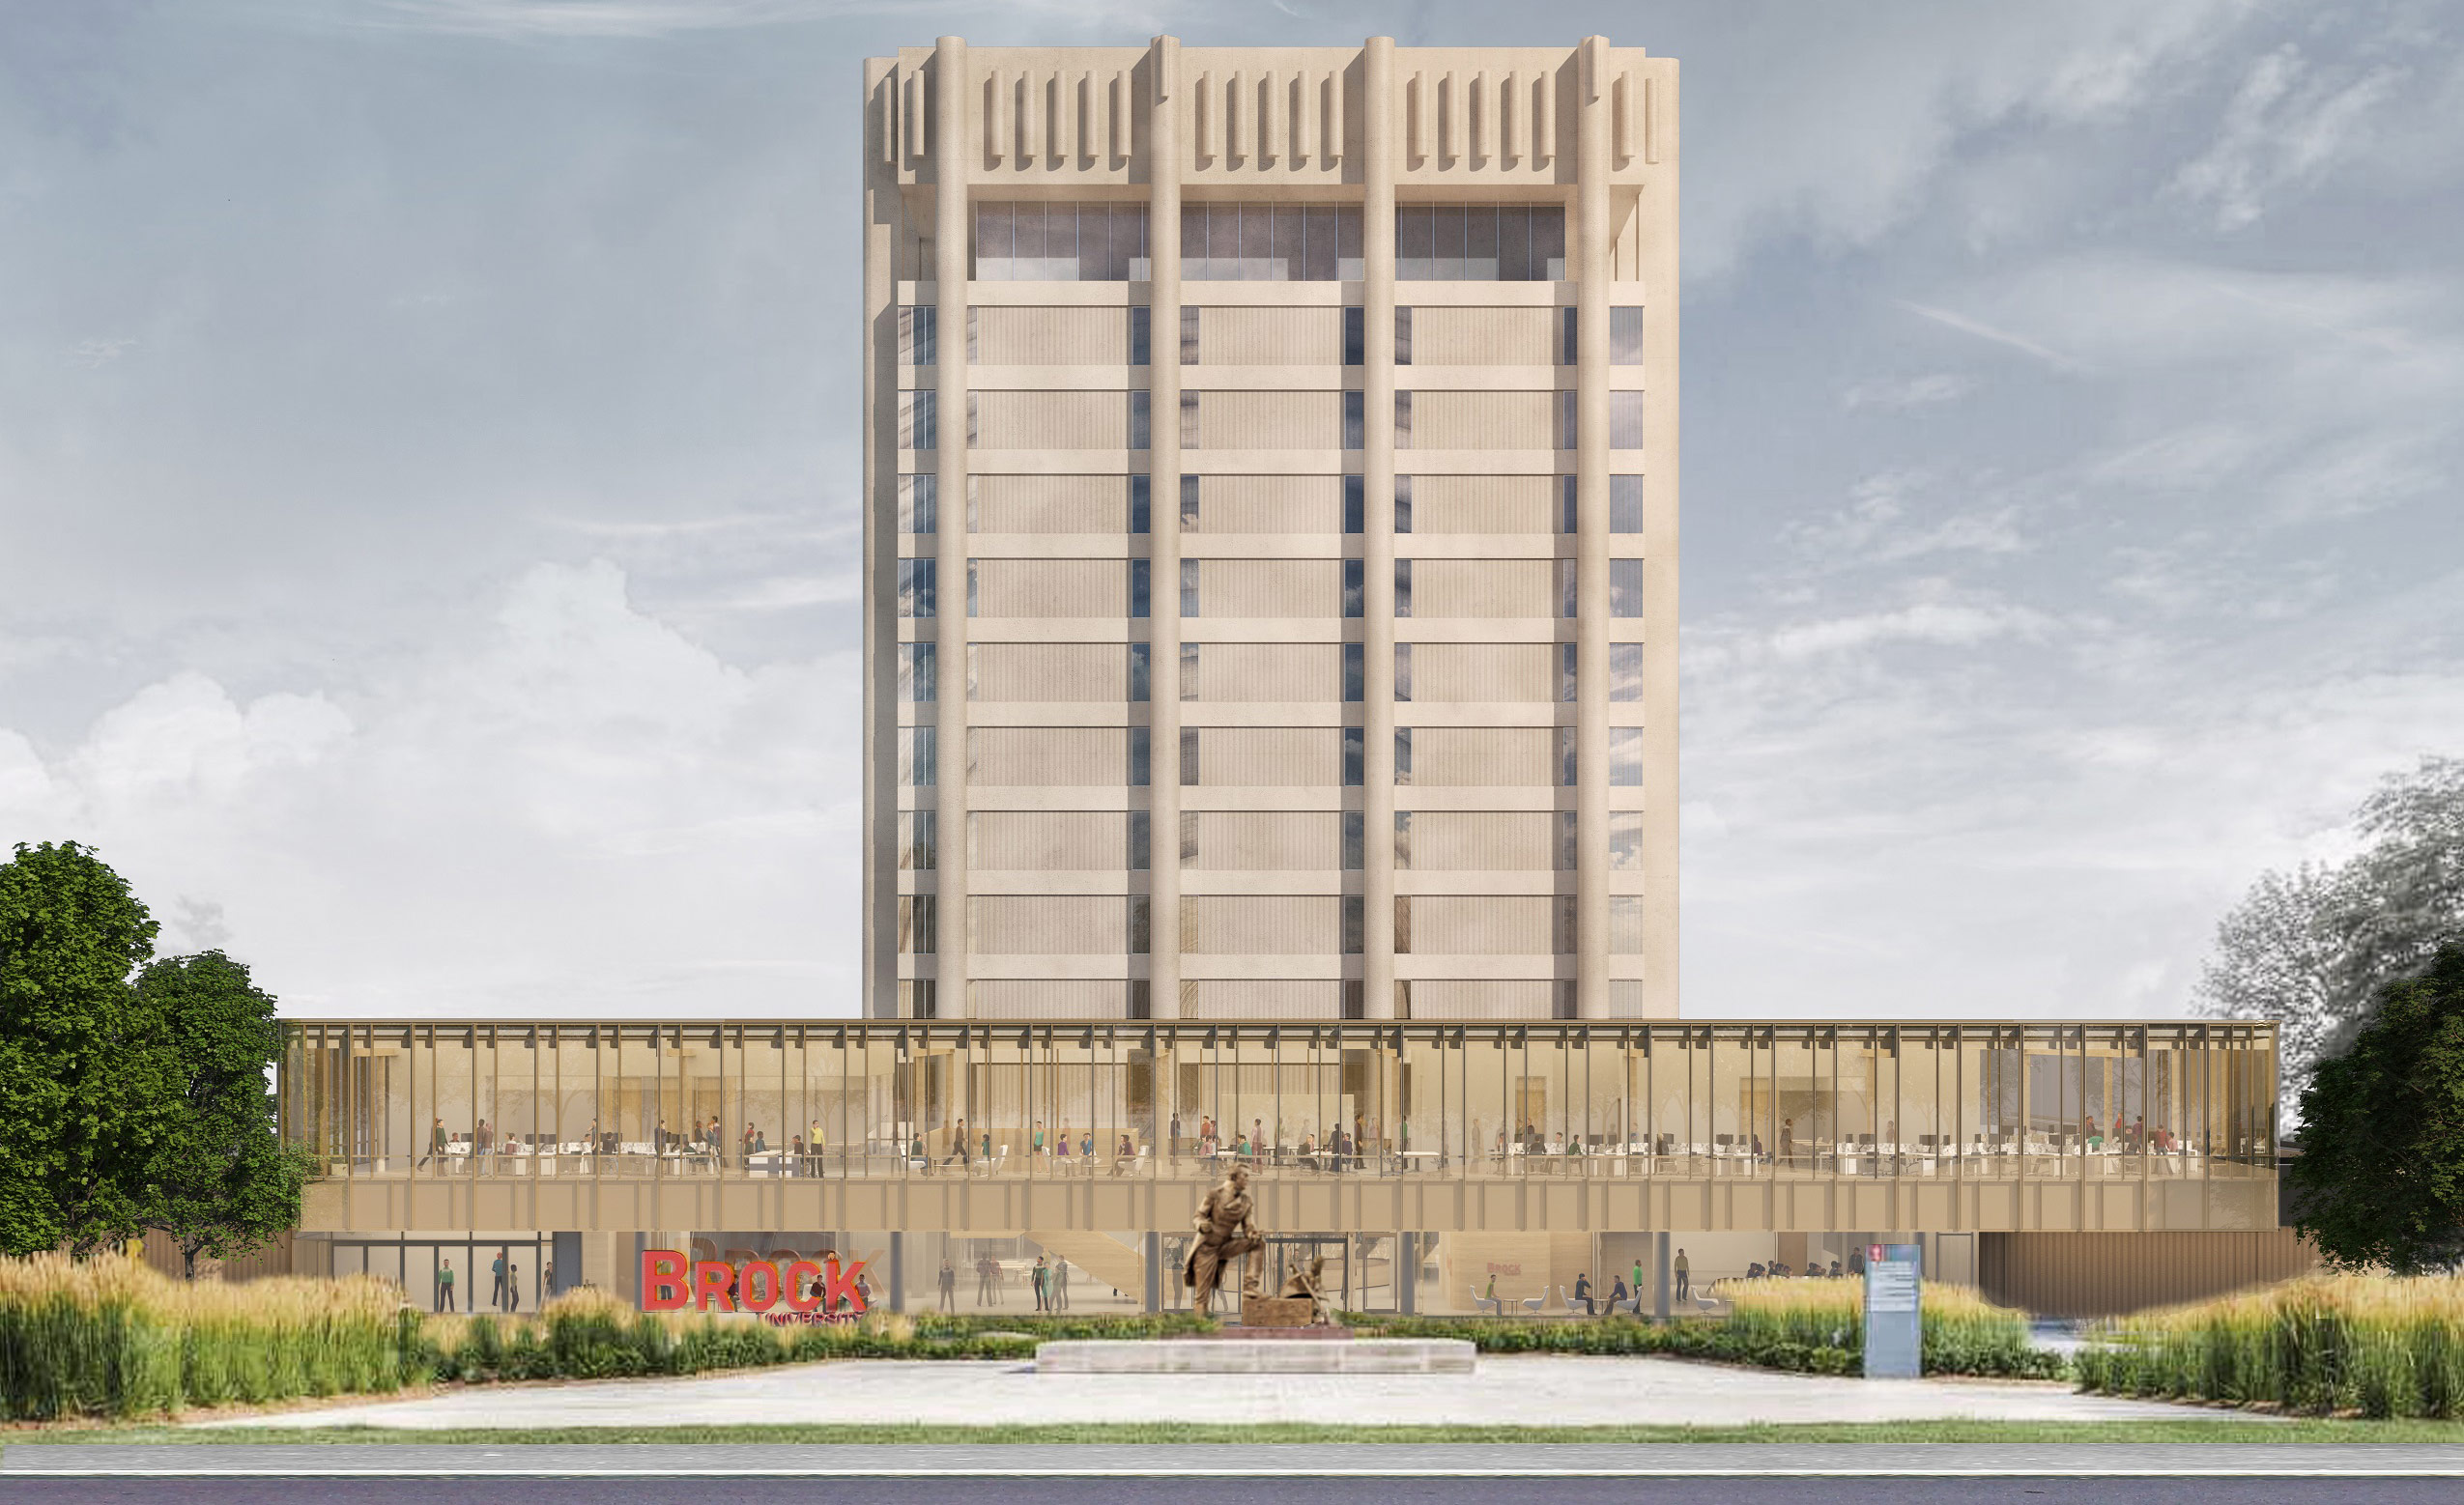
\includegraphics[scale=0.05]{Figures/Brock-LINC-Project-South-Elevation.jpg}
            \caption{Caption.}
            \label{fig:label2}
        \end{figure}
    \end{column}
\end{columns}

    \begin{itemize}
        \item Linear function: 
        \begin{equation}
            y=aX+b
        \end{equation}
    \end{itemize}
\end{frame}

\begin{frame}{Title}
    \begin{columns}[T] % align columns
\begin{column}{.5\textwidth}
Linear function: 
        \begin{equation}
            y=aX+b
        \end{equation}
Linear function: 
        \begin{equation}
            y=aX+b
        \end{equation}
\end{column}%
\hfill%
\begin{column}{.5\textwidth}
\begin{figure}
        \centering
        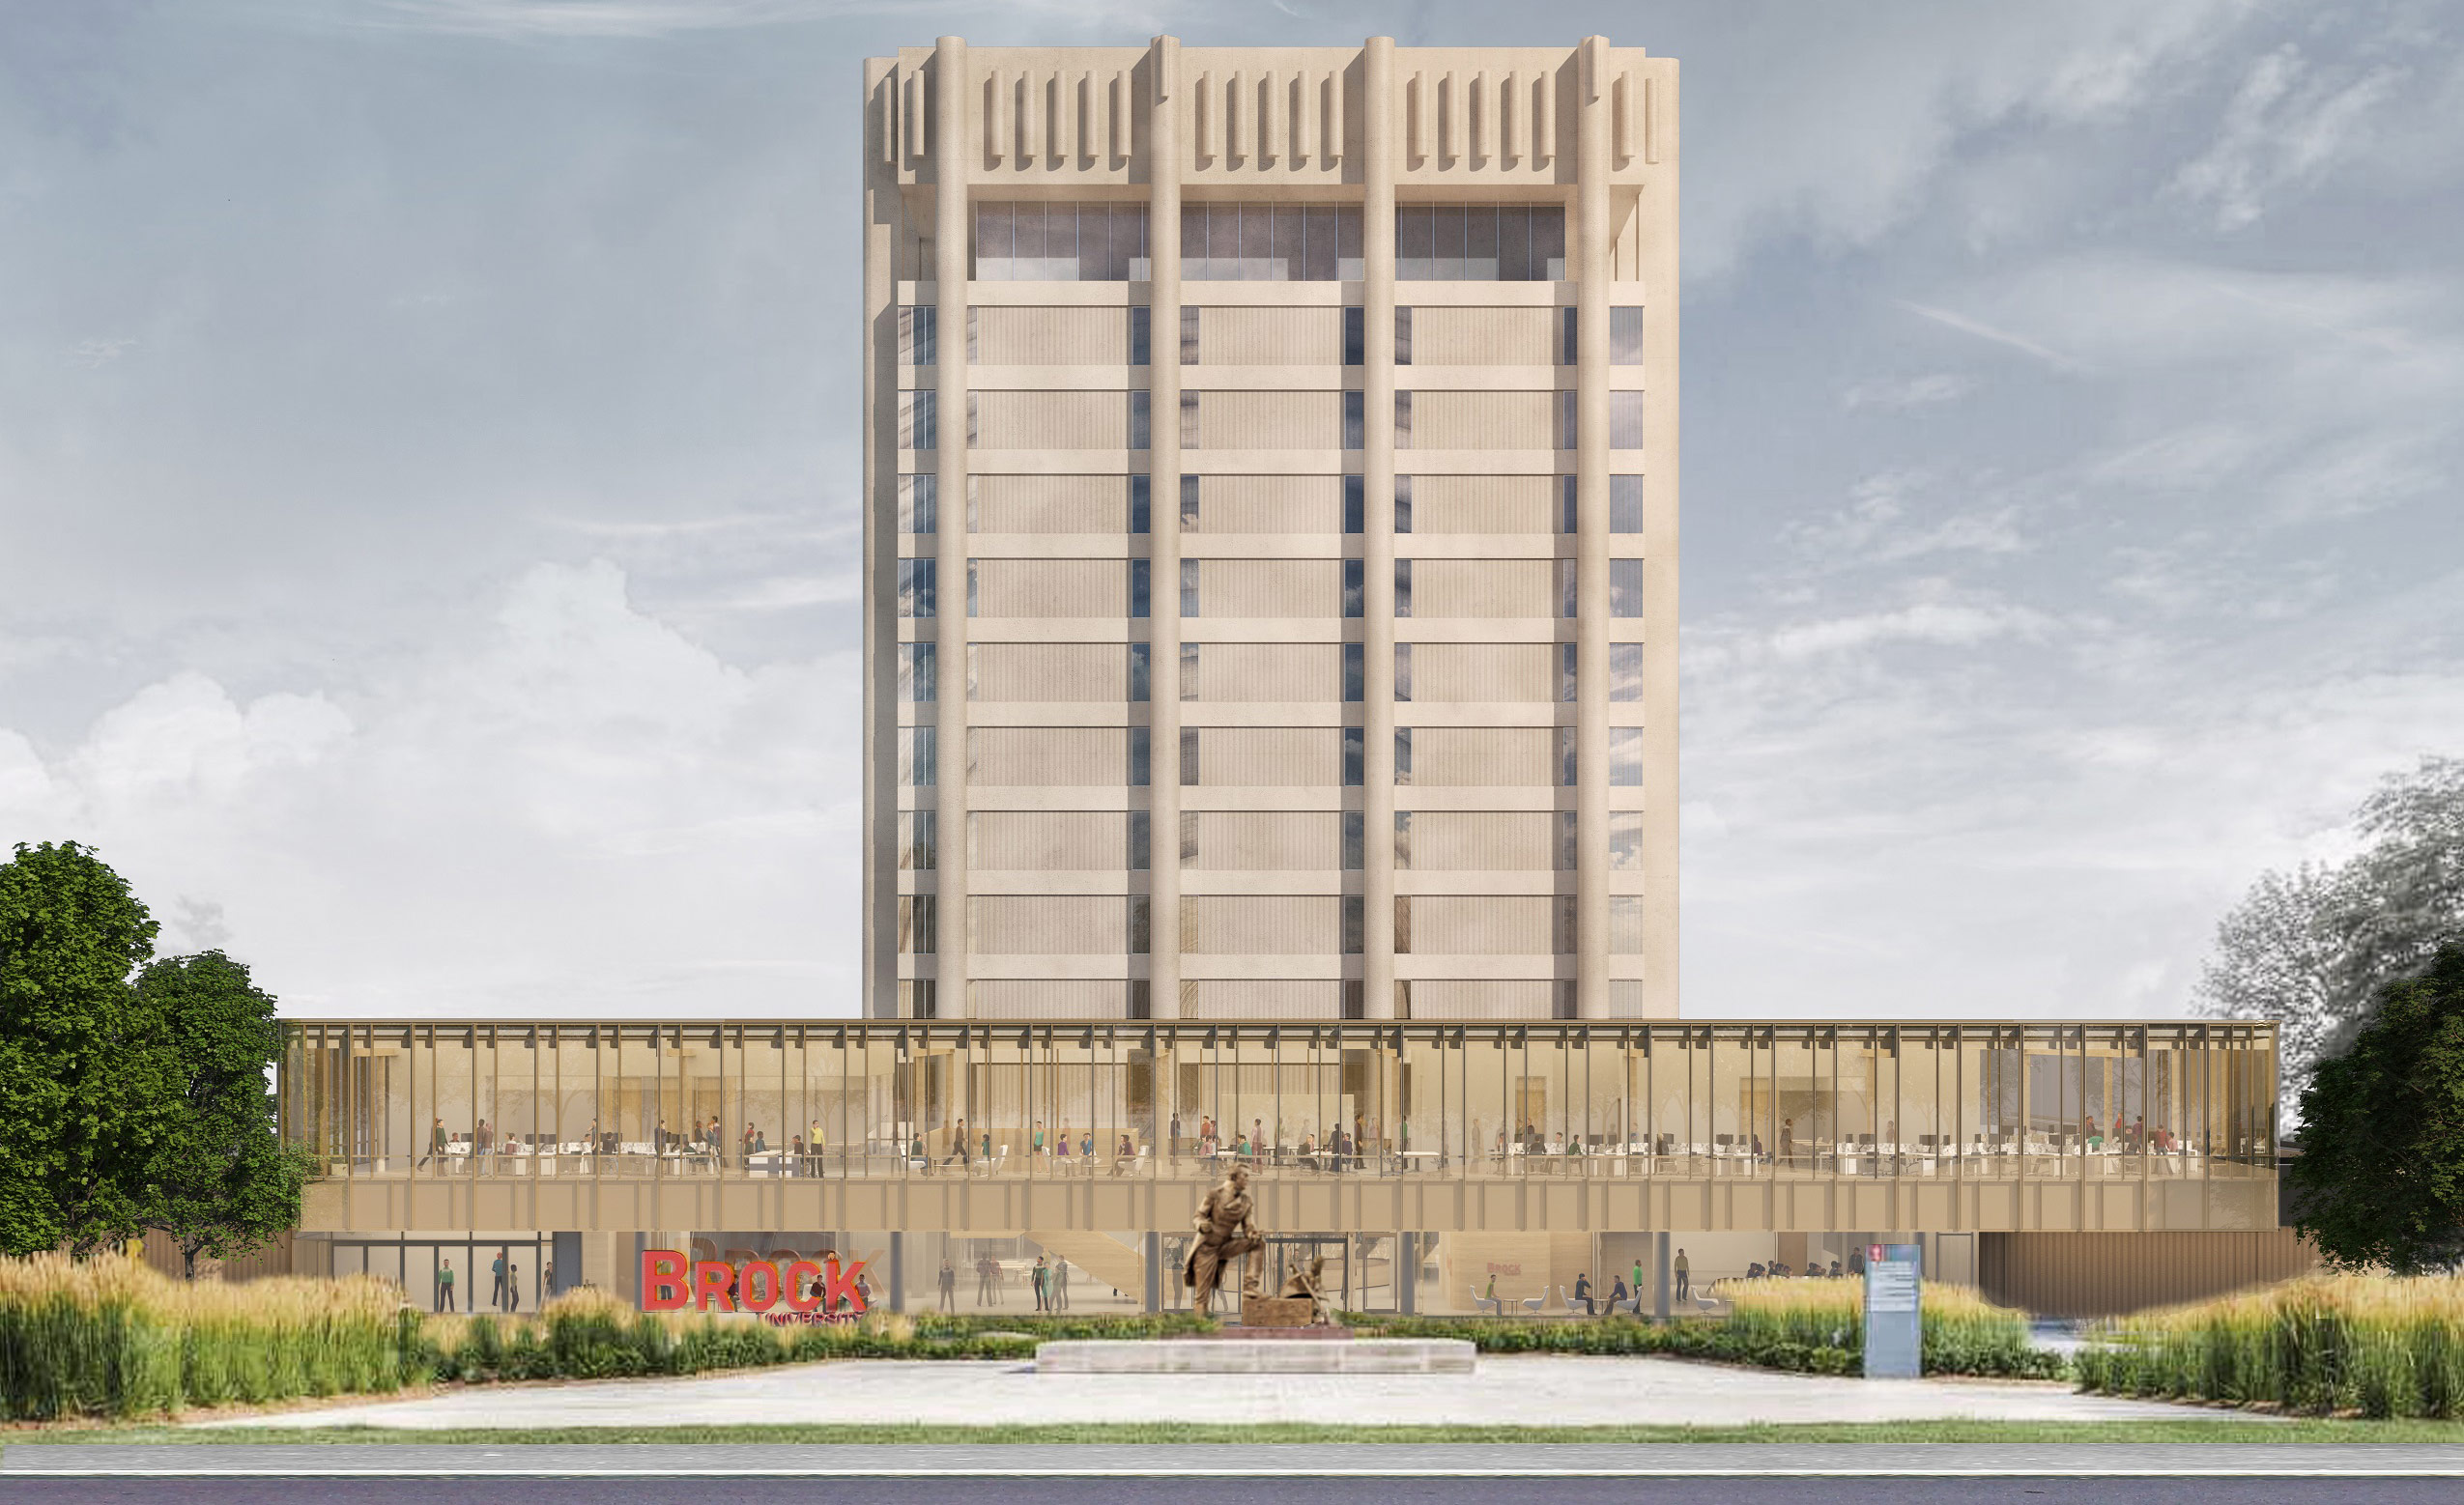
\includegraphics[scale=0.05]{Figures/Brock-LINC-Project-South-Elevation.jpg}
        \caption{Caption.}
        \label{fig:label4}
    \end{figure}
\end{column}%
\end{columns}
    
    
\end{frame}


\section{Section 3}
    \begin{frame}[plain]
        \vfill
      \centering
      \begin{beamercolorbox}[sep=8pt,center,shadow=true,rounded=true]{title}
        \usebeamerfont{title}\insertsectionhead\par%
        \color{blue}\noindent\rule{10cm}{1pt}
      \end{beamercolorbox}
      \vfill
  \end{frame}


\begin{frame}{Results}
    
    \begin{table}
        \centering
        \begin{tabular}{|c|c|c|c|c|} \hline 
            - & Col1 & Col2 & Col3 & Col4\\ \hline 
            Row2 & - & - & - & -\\ \hline 
            Row3 & -& -& -& \textbf{-}\\ \hline 
            Row4 & -& -& -& \textbf{-}\\ \hline 
            Row5 & -& -& -& -\\ \hline
        \end{tabular}
        \caption{Table.}
        \label{tab:table1}
    \end{table}
\end{frame}

\section{Conclusion}
    \begin{frame}[plain]
        \vfill
      \centering
      \begin{beamercolorbox}[sep=8pt,center,shadow=true,rounded=true]{title}
        \usebeamerfont{title}\insertsectionhead\par%
        \color{red}\noindent\rule{10cm}{1pt}
      \end{beamercolorbox}
      \vfill
  \end{frame}
  

\begin{frame}{Conclusion}
\begin{itemize}
    \item \lipsum[1][1]
    \item \lipsum[1][2]
    \item \lipsum[1][3]
    \item \lipsum[1][4]
\end{itemize}
\end{frame}


\begin{frame}[allowframebreaks]
        \frametitle{References}
\bibliographystyle{abbrv}
\bibliography{references}

\end{frame}

\section*{Thank you!}
    \begin{frame}[plain]
        \vfill
      \centering
      \begin{beamercolorbox}[sep=8pt,center,shadow=true,rounded=true]{title}
        \usebeamerfont{title}\insertsectionhead\par%
        \color{red}\noindent\rule{10cm}{1pt}
      \end{beamercolorbox}
      \vfill
  \end{frame}

\end{document}
